\chapter{WCDMA 移动通信系统}
\section{WCDMA 系统概述}
三种方案对比,详细见书P186。
\subsection{WCMDA的发展}
GSM->GPRS->EDGE->WCDMA->HSDPA->HSUPA>LET\\
详细演进版本可见P187。\\
\textbf{WCDMA }是从 GSM 演进而来,所以许多 WCDMA 的
高层协议和 GSM/GPRS 基本相同或相似,比如移
动性管理( MM )、 GPRS 移动性管理( GMM )、连
接管理( CM )以及会话管理( SM )等。\\
\textbf{移动终端}中通用用户识别模块( USIM )的
功能也是从 GSM 的用户识别模块( SIM )的功能
延伸而来的\\
\textbf{核心网是平滑的,但是空中接口发生了革命性的变化}
\subsection{WCMDA系统结构}
无线接入 网负责处理所有与无线通信相关的
功能。而 CN 则采用了 GSM/GPRS 的定义,这样可
以实现网络的平滑过渡,\textbf{核心网}负责对\textbf{话音及
数据业务进行交换和路由查找},以便将业务连
接至外部 网络.
\begin{figure}[H]
	\centering
	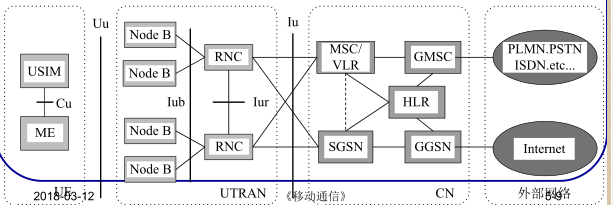
\includegraphics[width=0.7\linewidth]{figures/screenshot011}
	\caption{}
	\label{fig:screenshot011}
\end{figure}
\begin{enumerate}
	\item UE,UE 完成人与网络间的交互,通过\textbf{ Uu 接口}与无
	线接入网相连,与网络进行信令和数据交换。包
	括两部分:
	\begin{itemize}
		\item ME,移动设备
		\item USIM,UTMS用户识别模块。
	\end{itemize}
	\item 无线接入网(UTRAN),UTRAN 位于两个开放接口 Uu 和 Iu 之间,完成所有
	与无线有关的功能。
\textbf{	RAN由多个RNS组成,一个RNS由一个RNC和至少一个NOodeB组成。}
	\begin{itemize}
		\item 无线网络控制器( RNC ),主要完成连接建立和断开、切换、宏分集合并
		和\textbf{无线资源管理控制}等功能。
		\begin{enumerate}
			\item 控制 RNC ( CRNC )。对于某个 Node B 来说,直接
			控制它的 RNC 就是\textbf{控制} RNC ( CRNC )
			\item 服务 RNC(SRNC) 。与 CN 有连接,为 UE 提供资源的
			RNC。(越区切换合并)
			\item 漂移 RNC(DRNC) 。把自己的资源借给 SRNC 为某一
			个 UE 使用的(仅一个Node B资源)
		\end{enumerate}
		\begin{figure}[H]
			\centering
			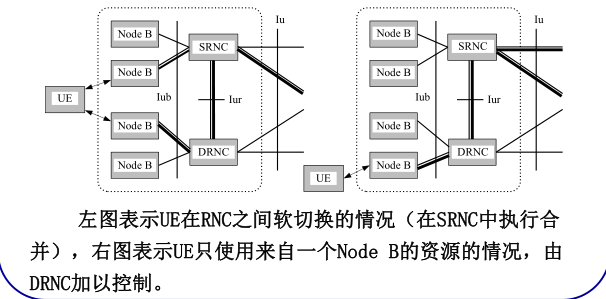
\includegraphics[width=0.7\linewidth]{figures/screenshot012}
			\caption{}
			\label{fig:screenshot012}
		\end{figure}
		\item Node B,Node B 通过 Iub 接口和基站控制器 RNC 互连。它主
		要由接口电路、基带处理单元、射频前端和控制单元
		部分组成。\textbf{ Node B=BBU(基带处理)+RRU(射频前端+ 天馈系统},\textbf{基带处理是核心功能},Node B 还负责完成更软切换、定位测量和执行无
		线资源分配与管理控制指令的功能
	\end{itemize}
	\item  CN 核心网络。
	\begin{itemize}
		\item CS域:MSC/VLR,GMSC
		\item PS域:SGSN,GGSN,CG。
		\item HLR.
	\end{itemize}
	\item 接口
	\begin{enumerate}
		\item Cu,USIM和ME之间
		\item Uu,UE和UTRAN,是UMTS中最重要的开放接口之一。
		\item Iu,UTRAN和CN。
		\item Iur,RNC之间
		\item Iub,Node B之间。
	\end{enumerate}
\end{enumerate}
\subsection{CDMA扩频技术的优点}
\begin{enumerate}
	\item 抗干扰能力强,特别是抗窄带干扰;
	\item 可检测性低,不容易被侦破
	\item 具有多址能力,易于实现码分多址技术
	\item 可抗多径干扰
	\item 可抗频率选择性衰落
	\item 频谱利用率高,容量大
\end{enumerate}
\subsection{UTRAN 接口协议}
\subsubsection{结构图}
\begin{figure}[H]
	\centering
	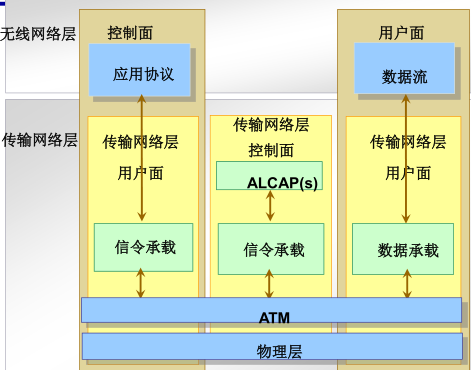
\includegraphics[width=0.7\linewidth]{figures/screenshot014}
	\caption{}
	\label{fig:screenshot014}
\end{figure}
特点:
\begin{enumerate}
	\item 所有接口具有开放性
	\item 将无线网络层与传输层分离
	\item 控制面和用户面分离
\end{enumerate}
Iu,Iub,Iur使用\textbf{ATM}承载。
\subsubsection{协议栈}
\textbf{UTRAN 控制面协议栈}是指协议和设备的对应关系
。 \textbf{UE 里面实现的协议是最完备}的,所有的 Node B 只实
现第一层,从 Uu 口的角度来讲,\textbf{ RNC 实现第二层(}从
MAC 到 RRC ),\textbf{ CN 只实现 RRC 之上的}
\begin{figure}[H]
	\centering
	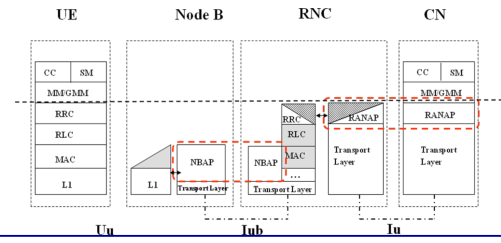
\includegraphics[width=0.7\linewidth]{figures/screenshot015}
	\caption{}
	\label{fig:screenshot015}
\end{figure}
\textbf{UTRAN 用户面协议栈:}用户面有 CS 和 PS 域,从 UE的角度讲,没有RRC。
\begin{figure}[H]
	\centering
	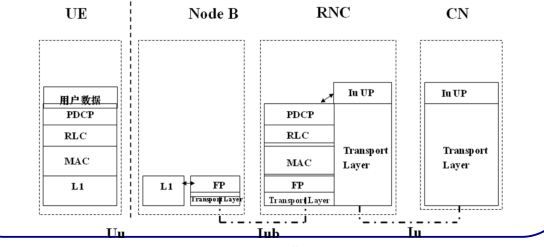
\includegraphics[width=0.7\linewidth]{figures/screenshot016}
	\caption{}
	\label{fig:screenshot016}
\end{figure}
\section{WCDMA系统的关键技术}
\begin{figure}[H]
	\centering
	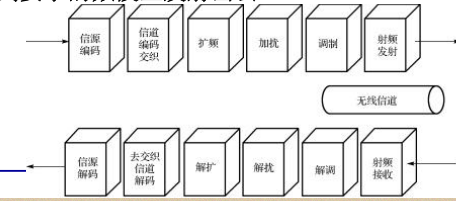
\includegraphics[width=0.7\linewidth]{figures/screenshot017}
	\caption{}
	\label{fig:screenshot017}
\end{figure}

\subsection{基本技术}
WCDMA 系统发射机和接收机的信号处理流程
\begin{enumerate}
	\item 信源编码 。自适应多 速率 AMR
	技术( 带8种信源 速率) .
	\item 信道编码 、交织:抵抗无线传播环境中的各种衰落。主要采用 卷积码(时延低,速率低)、 Turbo 码(时延高,速率高)和交
	织等信道编码技术
	\item 扩 频、加扰,这两步是 WCDMA 系统所特有的,采用高速的OVSF提高数
	\begin{itemize}
		\item 扩频:扩频又叫做信道化操作,用来区分来自\textbf{同一
		个信源的不同物理信道};采用高速的OVSF提高数
		字符号的速率,增加信号带宽。(良好的互相关,解决多址干扰)
		\item 加扰:采用Gold序列作为扰码,用以区分\textbf{不同的信
		源}。(良好的自相关,解决多径干扰)
	\end{itemize}
	字符号的速率,增加信号带宽
	\item 调制,
	\begin{itemize}
		\item 首先是将含有信息的基带信号调制至某一载波上
		\item 再通过上变频搬移至适合某信道传输的射频段
	\end{itemize}
\end{enumerate}
\subsection{RAKE接收}
\begin{itemize}
	\item 多径分离,Chip周期小于时延
	\item 多径合并准则,最强信号;等增益;最大比值合并
	\item  RAKE接收的本质:时间分集,多径分集
\end{itemize}
\subsection{功率控制技术}
功率控制的 \textbf{目的}:在 保证链路质量目标的前提下
使发射信号的功率最小 , 既减少 多址干扰 , 又可以
有效地防止 “ 远近效应 ” , 使系统维持高质量通信\\	
从通信链路的角度,功率控制可 分为
\begin{itemize}
	\item 前向功率控制,基站到移动台
	\item 反向功率控制,移动台到基站
\end{itemize}
从 功率控制方法的角度,功率控制可 分为
\begin{itemize}
	\item 开环功率控制,无控制指令,补偿平均路径损耗和慢衰落。
	\item 闭环功率控制,有控制指令。 
\end{itemize}
快速 、准确的\textbf{功率 控制技术}是 保证 WCDMA 系统性
能的\textbf{核心 }技术。
\subsubsection{反向开环功率控制}
根据\textbf{接收到的前向链路信号的功率大小来调整自己的发射功率}。开环功率控制由于补偿信道中的\textbf{平均路径损耗及慢衰落},有一个很大的\textbf{动态范围}。\\
关键在于:假设了前向和反向链路的衰落情况一致。所以可以通过测量前向链路来调整MS的发射功率。这就导致了当前向和反向链路相互独立时,该方式有较大误差。(如FDD方式)。
开环功率控制只能起到粗略控制。
的作用 。\\
\textbf{功能}
\begin{itemize}
	\item 调整移动台初始接入时的发射功率
	\item 弥补由于路径 损耗和慢衰落造成 的衰减的变化 。
\end{itemize}
\subsubsection{反向闭环功率控制}
建立于开环功率控制之上,最开环功率控制进行校正。根据反向链路上移动台的信号强弱,产生功率控制指令,通过前向链路将功率指令发送给移动台,移动台根据该指令,在开环功率控制所选择发射功率的基础上,快速校正自己功率。克服\textbf{快衰落}。
\begin{itemize}
	\item 内环功率控制,基站测量移动台的移动台信号,与某个门限比较,进行发送相应的功率控制指令。
	\item 外环功率控制,根据信号质量(如误帧率)对内环门限进行调整。
\end{itemize}
\begin{figure}[H]
	\centering
	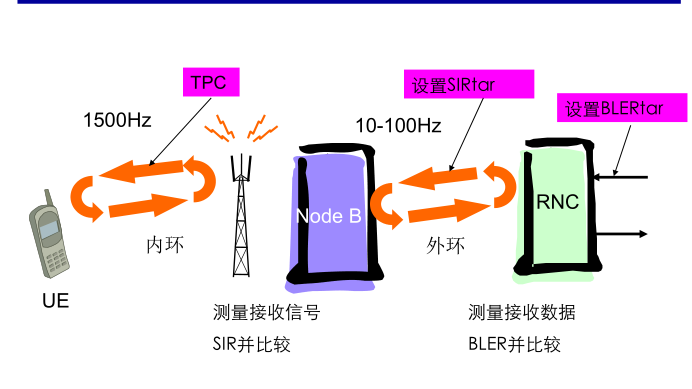
\includegraphics[width=0.7\linewidth]{figures/screenshot018}
	\caption{}
	\label{fig:screenshot018}
\end{figure}

\subsection{软切换}
\subsubsection{软切换}
在 CDMA 系统中,在同一个载波的不
同小区间进行的切换通常是软切换。上行链路软切换和更软切换的差别很大
\textbf{,两个基站接收移动台的码分信道,但接收到的数据
被发送到 RNC 进行合并}
\subsubsection{更软切换}
在上行链路方向,在基站的每个扇区
中接收移动台的码分信道,然后送入到\textbf{同一基带 Rake
接收机},并以通常的方式进行最大比值合并


\section{WCDMA的空中接口}
\subsection{分层结构}
\begin{figure}[H]
	\centering
	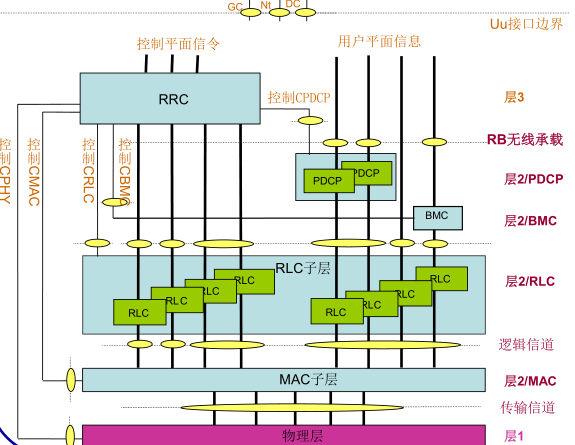
\includegraphics[width=0.7\linewidth]{figures/screenshot0019}
	\caption{}
	\label{fig:screenshot0019}
\end{figure}

\begin{description}
	\item[层3] 用户面用于用户数据的传输,控制面是RRC协议,重要职责是
	完成\textbf{UE和SRNC之间信令}的交互。
	\item[层2] 用户面和控制面数据 , 都
	需要经过 RLC 层和 MAC 层的处理 。
	\begin{itemize}
		\item 向上层提供无线承载
		\item PDCP和BMC只属于用户面
		\item RLC:将上层的PDU进行分割和重
		组、串联、填充,并完成WCDMA的
		加密功能
		\item MAC,实现逻辑信道和传输信道
		之间的映射和复用
	\end{itemize}
	\item[层1] 负责完成传输信道到物理信道的
	映射和复用;实现信道编码、交织、速率匹配、
	无线帧的分割、扩频调制和快速
	功率控制等功能
\end{description}
\subsection{无线资源控制层RRC}
\subsubsection{RRC层实现功能}
\begin{itemize}
	\item 一个 RRC 连接可以看作在 UE 和 SRNC 之间进行信令
	交互的一条逻辑通路,\textbf{每个 UE 最多只有一个 RRC 连接}。
	\item 对 UE 来说,没有 RRC 连接的状态称为空闲模式
	( IDLE ),有 RRC 连接的状态则称为 RRC
	\item UE 在空闲模式下\textbf{没有
	专用信道资源},只有通过
\textbf{公共控制信道}和 SRNC 之间
	传送 RRC	
\end{itemize}
\subsubsection{RAB 、 SRB 、 RB以及逻辑信道}
一个从 UE 到 CN 之间的承
载使用一个 RAB (无线接入承载)来定义,而 RB 则表
示其中从 UE 到 UTRAN ( SRNC )之间的一个无线承载,一个RAB可以对应于多个RB。一个RB又可分为:SRB,传送RRC信令,映射到DCCH。普通RB,传送用户面消息,映射到DTCH。
\subsection{空中接口的信道类型及其映射关系}
\subsubsection{无线接入承载RAB}
 UE 建立的每一个
呼叫都需要某种特定的
承载服务,RAB 可以形象地理解为 UE 和核心网间一个双向的数
据传输通道,这个数据传输通道可以看作由两部分构成
\begin{itemize}
	\item 一部分是 UE 与 RNC 之间 Uu 口的连接,即 RB ( RB 又细
	分为承载业务的 RB 和承载信令的 SRB )
	\item 另一部分就是 RNC 到核心网之间 Iu 口的 AAL2 连接。
\end{itemize}
\subsection{信道}
\begin{figure}[H]
	\centering
	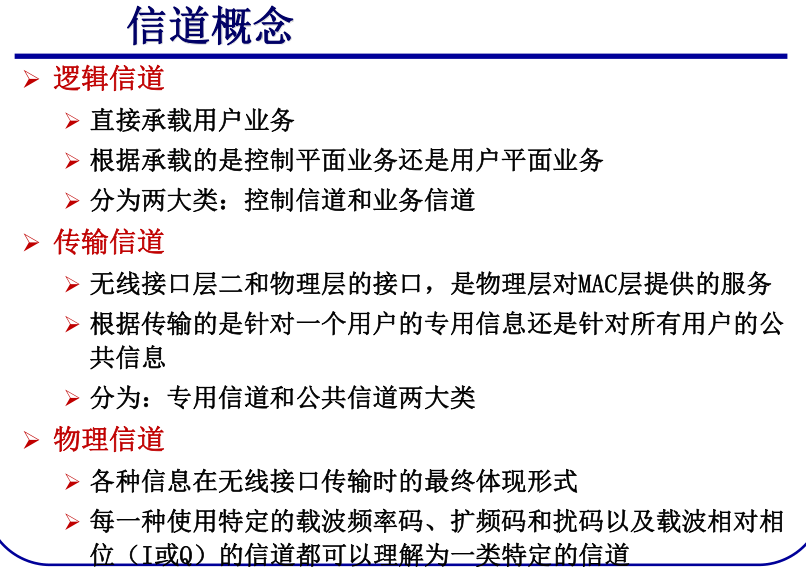
\includegraphics[width=0.7\linewidth]{figures/screenshot0020}
	\caption{}
	\label{fig:screenshot0020}
\end{figure}
